\documentclass[tikz,border=2pt]{standalone}
\usepackage{amsmath}
\usetikzlibrary{arrows.meta}
\begin{document}
% pay = 48 52 55 61 64 70 98 (thousand euros): min 48, first quartile 53.5, median 61, mean 64,
% third quartile 67, max 98; range() returns the end points 48 and 98.
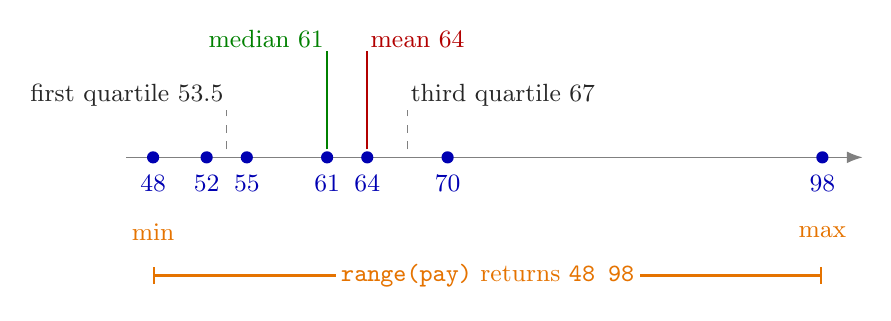
\begin{tikzpicture}[font=\small, >={Latex[length=2mm]}, x=0.17cm]
  \def\o{45}
  \draw[gray, ->] (46-\o,0) -- (101-\o,0);
  % data points
  \foreach \v in {48,52,55,61,64,70,98} {
    \fill[blue!70!black] (\v-\o,0) circle (2.2pt);
    \node[blue!70!black, below=3pt] at (\v-\o,0) {$\v$};
  }
  % markers
  \node[orange!90!black] at (48-\o,-0.95) {min};
  \node[orange!90!black] at (98-\o,-0.95) {max};
  \draw[gray, dashed] (53.5-\o,0.1) -- (53.5-\o,0.6);
  \node[gray!30!black, anchor=south east, inner sep=1pt] at (53.5-\o,0.6) {first quartile $53.5$};
  \draw[gray, dashed] (67-\o,0.1) -- (67-\o,0.6);
  \node[gray!30!black, anchor=south west, inner sep=1pt] at (67-\o,0.6) {third quartile $67$};
  \draw[green!50!black, thick] (61-\o,0.1) -- (61-\o,1.35);
  \node[green!50!black, anchor=south east, inner sep=1pt] at (61-\o,1.35) {median $61$};
  \draw[red!70!black, thick] (64-\o,0.1) -- (64-\o,1.35);
  \node[red!70!black, anchor=south west, inner sep=1pt] at (64-\o,1.35) {mean $64$};
  % range
  \draw[orange!90!black, |-|, thick] (48-\o,-1.5) -- (98-\o,-1.5);
  \node[orange!90!black, fill=white, inner sep=2pt] at (73-\o,-1.5) {\texttt{range(pay)} returns \texttt{48 98}};
\end{tikzpicture}
\end{document}
